\section{Case study: four prompt divergences on E4B}\label{sec:case}

\Cref{sec:conform} lists ways in which a local stack can send the model other prompts than the scorer does, and
\cref{sec:parity} shows that a comparison of 24 tasks cannot say whether such a divergence matters. This section
reports the experiment that can. It takes four divergences that we or public notebooks had actually run with, turns
each into one arm, and measures E4B's solved share against the scorer's path on 231 tasks with four repeats. The
design, the analysis and the power simulation were registered before the first job.

\Cref{sec:case-design} is the account of the short paper. The subsections after it give the full record: how the
block ran, every outcome count, the primary and secondary analyses with their sensitivity checks, how many requests
each divergence actually changed, and the exploratory measures of time and tokens. The rows are in the released
files \texttt{e8\_runs.csv}, \texttt{e8\_tasks.csv} and \texttt{e8\_repositories.csv}, and \cref{sec:app-recompute}
repeats the analysis with the released kit.

\subsection{Design and main result}\label{sec:case-design}

% written by scripts/reuse_short.py from the sources of the short paper; do not edit
Five arms share one model server, one withheld agent bundle, google-adk 1.36.1 and all sampling settings.

\begin{table}[!tb]
\centering
\caption{Arms; changes in percentage points.}\label{tab:casearms}
\footnotesize
\begin{tabular}{@{}
  >{\raggedright\arraybackslash}p{(\linewidth - 6\tabcolsep) * \real{0.0500}}
  >{\raggedright\arraybackslash}p{(\linewidth - 6\tabcolsep) * \real{0.4000}}
  >{\raggedright\arraybackslash}p{(\linewidth - 6\tabcolsep) * \real{0.1900}}
  >{\raggedright\arraybackslash}p{(\linewidth - 6\tabcolsep) * \real{0.3600}}@{}}
\toprule
\begin{minipage}[b]{\linewidth}\raggedright
Arm
\end{minipage} & \begin{minipage}[b]{\linewidth}\raggedright
Difference from the scorer path
\end{minipage} & \begin{minipage}[b]{\linewidth}\raggedright
Requests changed by the divergence
\end{minipage} & \begin{minipage}[b]{\linewidth}\raggedright
Change against F {[}95\% interval{]}; Holm p
\end{minipage} \\
\midrule
F & none: role \texttt{tool}, Kaggle template, compaction at 14,336 tokens, thoughts under both keys & --- & solve rate 23.8\% \\
R & model name contains ``gemma4'': tool results get role \texttt{tool\_responses} & 89\% & \ensuremath{-}0.3 {[}\ensuremath{-}2.8, +2.2{]}; p = 1 \\
C & compaction unset: prompts grow until rejected above 24,576 tokens (the run ends; edits are still graded) & 21\% & +0.2 {[}\ensuremath{-}2.0, +2.5{]}; p = 1 \\
H & history thoughts removed from every request, as when a client omits the key the server reads & 90\% & \ensuremath{-}2.1 {[}\ensuremath{-}4.4, +0.4{]}; p = 0.44 \\
T & the Hugging Face E4B template: a thought opener is forced after each tool result & 85\% & +0.8 {[}\ensuremath{-}1.4, +2.9{]}; p = 1 \\
\bottomrule
\end{tabular}
\end{table}

No newline arm was run: both templates render it identically on this server.

\paragraph{Panel.} Removing tasks used by other panels, reserved repositories, slow tasks and duplicates from the 579 leaves 231 tasks in 15 repositories. They run 4 repeats in 5 arms (4,620 jobs); for each task and repeat the arms run back to back in counterbalanced order.

\textbf{Analysis, frozen before any outcome} (protocol sha256 \texttt{\seqsplit{070c9655d96372d054f430727259de7b25af2ca93c3ec4c9295dfdc37aeb8cf4}}). The estimand $d_X$ is the mean over tasks of arm X's solve rate minus arm F's. The primary test is an exact two-sided task-level sign-flip test, Holm-corrected over the four arms at 0.05; only then do we say that X raises or lowers E4B's solve rate \emph{on these tasks}. Intervals (unadjusted) invert that test. A repository-cluster bootstrap interval is secondary (lower simulated power). A frozen checker re-renders every returned request from the job's dump, matches the server's token count and confirms the job's arm; a failing job is re-run. Outcomes stayed blind until a pre-registered cut-off (2026-11-11 06:00 UTC) and were unblinded once.

\paragraph{Power, simulated before data.} The family-wise false-claim rate is 1.2--4.2\%. At 231 tasks an even 5-point drop in one arm is detected with probability 82--100\% across the simulated settings; the drop or gain detected with 80\% power ranges from below 3 to about 5.2 points.

\paragraph{Deviations recorded blind.} Independent validation of the final runner finished only after launch. From about an hour in, a second workload held about 9.6 GiB of GPU memory, so timings are under mixed load. The block stopped three times: after 967 jobs at the runner's open-file limit (cause unknown), after 378 more by an external termination signal on the shared machine, and after 3,074 more when the kernel's out-of-memory killer ended the model server (cause undiagnosed). Each resume ran only never-started jobs; the 24 interrupted jobs were re-run once.

\paragraph{Results.} All jobs finished before the cut-off. Every arm has a valid row in 924 of 924 slots, and the checker passed all 4,620 analysed jobs. No pre-emption was recorded; 6.0\% of runs took over 240 s, above the pre-registered 5\% threshold. No difference from F was detected for any arm (Table~\ref{tab:casearms}, Figure~\ref{fig:parity}B; smallest Holm-adjusted p 0.44); the secondary repository-cluster intervals all include zero. The largest estimate is H's \ensuremath{-}2.1 points (unadjusted p 0.11; \ensuremath{-}1.3 with time-limit rows as missing). In exploratory measures, H runs averaged 137 s against 78 s and ended unsolved at the bundle's five-minute limit in 11.5\% of runs against 1.8\%; in C, 12.3\% of runs ended unsolved on a rejected over-long prompt. These are null results, not evidence of no effect: the simultaneous 98.75\% intervals allow a drop of 5.1 points (H) and a gain of 3.5 (T).

\begin{figure}[!tb]
\centering
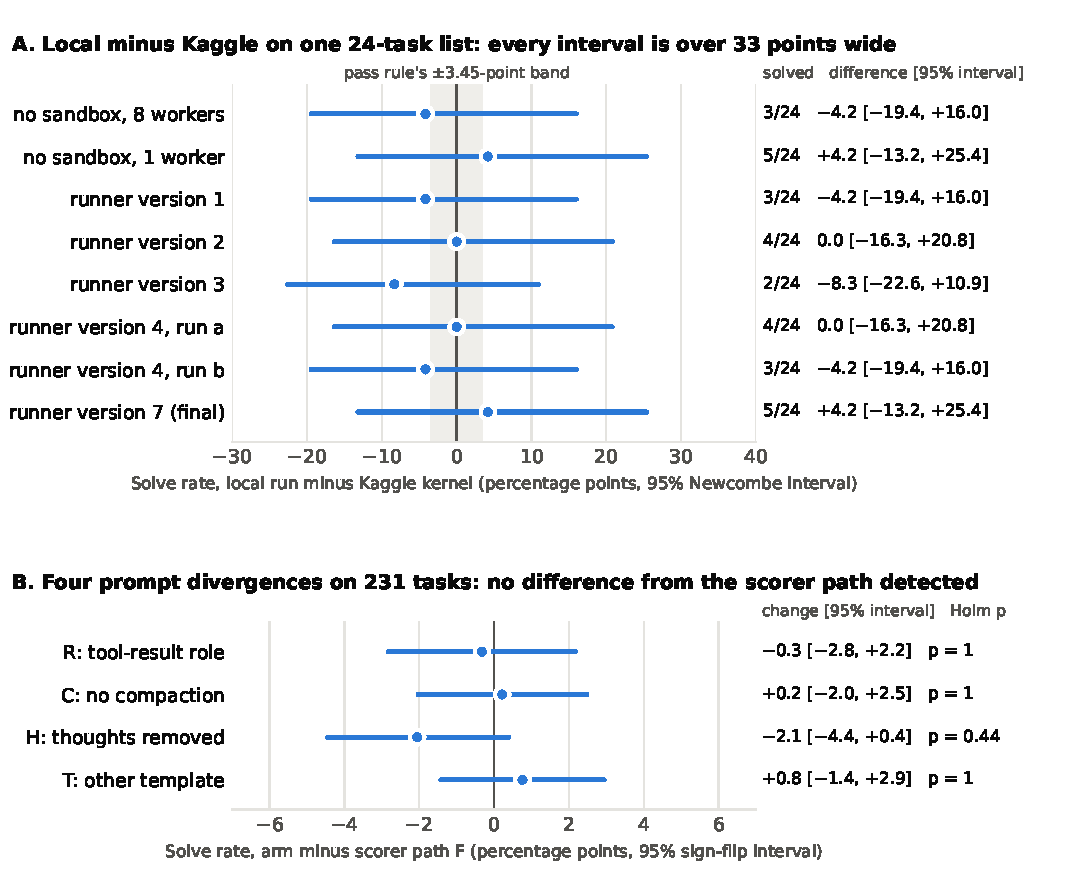
\includegraphics[width=\linewidth]{fig/parity_effects.pdf}
\caption{(A) Solve-rate difference, local minus Kaggle (pooled 8/48), for eight local runs of one 24-task list (95\% Newcombe intervals, runs treated as independent); shaded: the pass rule's \ensuremath{\pm}3.45 points. (B) Change in solve rate against F on 231 tasks: estimates, 95\% intervals and Holm-adjusted p.}\label{fig:parity}
\end{figure}


% written by scripts/reuse_short.py from the sources of the short paper; do not edit
\subsection{Execution record}

The first job started on \SFirstStart{} UTC and the last one ended on \SLastEnd{} UTC, before the cut-off
(2026-11-11 06:00 UTC). The block ran as four batches and one batch of re-runs (Table~\ref{tab:s-batches}). Three
batches stopped early, for the reasons in the last column, and each following batch started only jobs that had never
started. In all, \SJobsStarted{} jobs were started: the \SAgentRows{} analysed runs and \SInfraRowsAll{} interrupted
jobs. Of the interrupted jobs, \SInfraRowsWritten{} left an infrastructure row; the other \SInfraNoRow{}, all in
batch~1, left none and are counted from the list of started jobs. Each interrupted slot was re-run once, so every slot
has exactly one analysed run. The released file holds every written row.

\begin{table}[!htb]
\centering
\caption{Execution record: the block ran as four batches and one batch of re-runs. An interrupted job is an infrastructure row, with or without a written result row; its slot was re-run once.}\label{tab:s-batches}
\footnotesize
\begin{tabular}{rrrrrl}
\toprule
Batch & \parbox[b]{1.2cm}{\raggedleft Jobs started} & \parbox[b]{1.4cm}{\raggedleft Analysed runs} & \parbox[b]{1.9cm}{\raggedleft Interrupted, row written} & \parbox[b]{1.9cm}{\raggedleft Interrupted, no row} & How the batch ended \\
\midrule
1 & 967 & 959 & 0 & 8 & runner reached its open-file limit \\
2 & 378 & 370 & 8 & 0 & external termination signal \\
3 & 3{,}074 & 3{,}066 & 8 & 0 & model server ended (out of memory) \\
4 & 201 & 201 & 0 & 0 & job list completed \\
5 & 24 & 24 & 0 & 0 & re-runs of the interrupted jobs completed \\
\bottomrule
\end{tabular}
\end{table}


\SLoadAbove{} of the \SLoadRows{} runs (\SLoadShare\%) took more than \SLoadThreshold{}~s of agent time. This is above
the \SLoadFlag\% share that the protocol set as the sign of a loaded machine: from about an hour into the block a
second workload held part of the memory of the GPU (\cref{sec:case-design}), so the times are under mixed load. No pre-emption
was recorded.

\subsection{Outcomes and solve rates}

Table~\ref{tab:s-outcomes} splits the runs of each arm by how they ended and Table~\ref{tab:s-rates} gives the solve
rates, which lie between \SMinRate\% and \SMaxRate\%. Two arms end differently from F. In C, \SCRejected{} runs
(\SCRejectedShare\%) ended unsolved because a prompt grew past the server's limit and was rejected; no F run ended
this way, and \SFCompactedShare\% of the F runs made at least one history summary. In H, \SHUnsolvedAtLimit{} runs
(\SHUnsolvedAtLimitShare\%) were unsolved at the bundle's five-minute limit, against \SFUnsolvedAtLimit{}
(\SFUnsolvedAtLimitShare\%) in F.

\begin{table}[!htb]
\centering
\caption{Outcome of every analysed run, by arm (one row per task, arm and repeat).}\label{tab:s-outcomes}
\footnotesize
\begin{tabular}{lrrrrrrr}
\toprule
Arm & \parbox[b]{1.75cm}{\raggedleft Solved} & \parbox[b]{1.75cm}{\raggedleft Unsolved, run completed} & \parbox[b]{1.75cm}{\raggedleft Five-minute limit} & \parbox[b]{1.75cm}{\raggedleft Over-long prompt rejected} & \parbox[b]{1.75cm}{\raggedleft Tool-call budget (28)} & \parbox[b]{1.75cm}{\raggedleft No submission} & Runs \\
\midrule
F & 220 & 676 & 17 & 0 & 6 & 5 & 924 \\
R & 217 & 677 & 20 & 0 & 9 & 1 & 924 \\
C & 222 & 568 & 17 & 114 & 1 & 2 & 924 \\
H & 201 & 597 & 106 & 1 & 18 & 1 & 924 \\
T & 227 & 668 & 19 & 0 & 4 & 6 & 924 \\
\bottomrule
\end{tabular}

\par\smallskip\parbox{0.96\linewidth}{\footnotesize Only the runs of the first column are solved; the other columns split the unsolved runs by how the run ended. A run that ended at a limit was still graded on the edits it had made: 5 solved runs lasted the full five minutes (all in arm H), and 86 of the 179 runs unsolved at that limit had left edits that were tested.}
\end{table}

\begin{table}[!htb]
\centering
\caption{Solve rate per arm: task-weighted mean with a 95\% interval from a repository-clustered (CR1) standard error; solved runs per repeat.}\label{tab:s-rates}
\footnotesize
\begin{tabular}{lrrrrrrrr}
\toprule
Arm & Solve rate (\%) & 95\% interval & Solved runs & Repeat 1 & 2 & 3 & 4 & Runs \\
\midrule
F & 23.81 & [16.7, 30.9] & 220 & 50 & 59 & 57 & 54 & 924 \\
R & 23.48 & [17.7, 29.3] & 217 & 53 & 53 & 54 & 57 & 924 \\
C & 24.03 & [16.6, 31.5] & 222 & 58 & 56 & 55 & 53 & 924 \\
H & 21.75 & [15.9, 27.6] & 201 & 50 & 49 & 54 & 48 & 924 \\
T & 24.57 & [18.6, 30.5] & 227 & 59 & 56 & 51 & 61 & 924 \\
\bottomrule
\end{tabular}
\end{table}


Table~\ref{tab:s-taskhist} shows why a difference between arms is hard to detect on this panel: \STasksNever{} of the
\STasks{} tasks were solved in no run of any arm and \STasksAlways{} in every run, so the other \STasksMixed{} tasks
carry every difference.

\begin{table}[!htb]
\centering
\caption{Tasks by the number of solved repeats (of four), per arm.}\label{tab:s-taskhist}
\footnotesize
\begin{tabular}{lrrrrrr}
\toprule
Arm & 0 solved & 1 solved & 2 solved & 3 solved & 4 solved & Tasks \\
\midrule
F & 149 & 16 & 21 & 18 & 27 & 231 \\
R & 152 & 14 & 21 & 15 & 29 & 231 \\
C & 151 & 15 & 18 & 17 & 30 & 231 \\
H & 155 & 21 & 13 & 14 & 28 & 231 \\
T & 151 & 14 & 13 & 25 & 28 & 231 \\
\bottomrule
\end{tabular}

\par\smallskip\parbox{0.96\linewidth}{\footnotesize 135 of the 231 tasks were solved in no run of any arm (0 of 20 runs) and 13 in every run; the other 83 tasks carry every difference between arms.}
\end{table}


\subsection{Primary analysis: tasks}

For a task, let $K$ be the number of solved repeats in the arm minus the number in F, from $-4$ to $+4$. The estimate
$d$ is the mean of $K/4$ over the \STasks{} tasks. Under the null hypothesis the arm and F are exchangeable within a
task, so each $K$ is as likely to carry one sign as the other; the test compares $|\sum K|$ with its distribution
over all sign assignments, computed exactly. Holm's method adjusts the four $p$-values. The intervals invert the same
test under a constant shift, with \SReproDraws{} frozen Monte Carlo sign draws.

No difference from F was detected for any arm (Table~\ref{tab:s-primary}, Figure~\ref{fig:s-taskdiff}). In every arm
between \SNoDifferMin{} and \SNoDifferMax{} of the \STasks{} tasks have the same number of solved repeats as in F. The
largest estimate is that of H: \SHTasksDown{} tasks have fewer solved repeats than in F and \SHTasksUp{} have more,
which gives $-\SHd$ points with exact $p = \SHp$ and Holm-adjusted $p = \SHHolm$. These are null results, not
evidence of no effect. The simultaneous 98.75\% intervals show what the experiment cannot exclude: a drop of up to
\SHSimLo{} points (H) and a gain of up to \STSimHi{} points (T).

\begin{table}[!htb]
\centering
\caption{Primary analysis: change in solve rate against F in percentage points, tasks with fewer and with more solved repeats than in F, exact two-sided task-level sign-flip test, Holm adjustment over the four arms, and intervals from inverting the test.}\label{tab:s-primary}
\footnotesize\setlength{\tabcolsep}{4pt}
\begin{tabular}{lrrrrrrrr}
\toprule
Arm & $d$ & Exact $d$ & \parbox[b]{1.5cm}{\raggedleft Tasks lower; higher} & Exact $p$ & Holm $p$ & \parbox[b]{1.7cm}{\raggedleft Monte Carlo $p$} & 95\% interval & 98.75\% simultaneous \\
\midrule
R & ${-}0.32$ & ${-}1/308$ & 26; 33 & 0.8652 & 1.000 & 0.8650 & [${-}2.82$, ${+}2.17$] & [${-}3.51$, ${+}2.85$] \\
C & ${+}0.22$ & $1/462$ & 26; 22 & 0.9253 & 1.000 & 0.9243 & [${-}2.03$, ${+}2.48$] & [${-}2.65$, ${+}3.09$] \\
H & ${-}2.06$ & ${-}19/924$ & 34; 20 & 0.1102 & 0.441 & 0.1106 & [${-}4.45$, ${+}0.38$] & [${-}5.09$, ${+}0.95$] \\
T & ${+}0.76$ & $1/132$ & 25; 30 & 0.5604 & 1.000 & 0.5599 & [${-}1.42$, ${+}2.94$] & [${-}2.02$, ${+}3.54$] \\
\bottomrule
\end{tabular}
\end{table}


\begin{figure}[!htb]
\centering
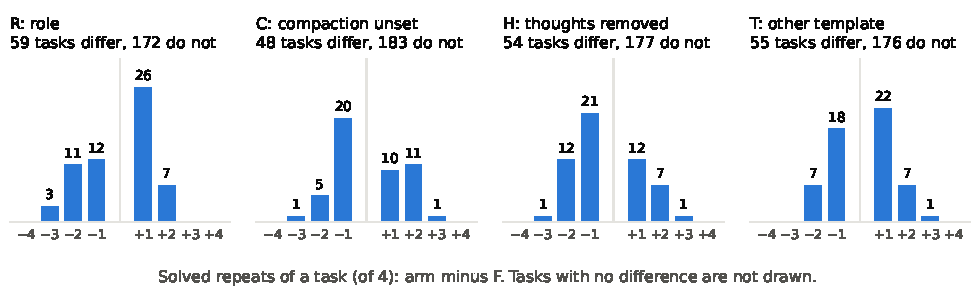
\includegraphics[width=\linewidth]{fig/supp_taskdiff.pdf}
\caption{Tasks whose number of solved repeats differs between an arm and F. Bars to the left of the centre line are
tasks with fewer solved repeats in the arm.}
\label{fig:s-taskdiff}
\end{figure}

\subsection{Secondary analysis: repositories}

Tasks of one repository tend to succeed and fail together, so the registered secondary analysis takes the \SRepos{}
repositories as its units (Table~\ref{tab:s-repolevel}). Table~\ref{tab:s-repos} and Figure~\ref{fig:s-repos} show
each repository. All four repository-level intervals include zero, and the smallest two-sided $p$ is \SMinRepoP{} (H).
The leave-one-repository-out estimates of H stay negative ($-\SHLooLo$ to $-\SHLooHi$ points), so no single
repository produces the estimate of H; those of R, C and T change sign.

\begin{table}[!htb]
\centering
\caption{Secondary analysis at the repository level (15 repositories): exact wild cluster bootstrap-$t$ with Rademacher weights, its inverted 95\% interval, the six-point (Webb) variant, a CR1 interval, the repository-equal estimate and the range of leave-one-repository-out estimates. Estimates in percentage points.}\label{tab:s-repolevel}
\footnotesize\setlength{\tabcolsep}{4pt}
\begin{tabular}{lrrrrrrr}
\toprule
Arm & \parbox[b]{1.9cm}{\raggedleft Repositories that differ} & Exact $p$ & Webb $p$ & 95\% interval & CR1 interval & \parbox[b]{1.9cm}{\raggedleft Repository-equal} & Leave-one-out range \\
\midrule
R & 12 & 0.8188 & 0.7780 & [${-}3.81$, ${+}2.38$] & [${-}2.70$, ${+}2.05$] & ${+}1.62$ & [${-}1.09$, ${+}0.36$] \\
C & 8 & 0.8438 & 0.7788 & [${-}0.88$, ${+}2.81$] & [${-}1.22$, ${+}1.65$] & ${+}4.02$ & [${-}0.22$, ${+}0.60$] \\
H & 12 & 0.1831 & 0.1736 & [${-}4.94$, ${+}1.56$] & [${-}4.65$, ${+}0.53$] & ${-}2.98$ & [${-}3.01$, ${-}1.44$] \\
T & 9 & 0.8047 & 0.7374 & [${-}1.44$, ${+}4.62$] & [${-}2.09$, ${+}3.61$] & ${+}2.65$ & [${-}0.55$, ${+}1.66$] \\
\bottomrule
\end{tabular}
\end{table}

\begin{table}[!htb]
\centering
\caption{The 15 repositories of the panel: tasks, runs solved in arm F (of four per task) and, per arm, the summed change against F in task-equivalents (solved runs divided by four).}\label{tab:s-repos}
\footnotesize
\begin{tabular}{lrrrrrr}
\toprule
Repository & Tasks & F solved runs & R & C & H & T \\
\midrule
\texttt{pypa/packaging} & 65 & 65 of 260 & ${+}0.50$ & ${-}0.50$ & ${-}2.00$ & ${-}1.00$ \\
\texttt{pydantic/pydantic-settings} & 48 & 27 of 192 & ${+}1.25$ & 0 & ${+}0.75$ & ${+}2.75$ \\
\texttt{python-poetry/tomlkit} & 35 & 31 of 140 & ${-}1.00$ & ${-}0.50$ & ${-}1.50$ & 0 \\
\texttt{more-itertools/more-itertools} & 23 & 39 of 92 & ${-}1.50$ & ${+}0.25$ & ${-}1.75$ & 0 \\
\texttt{pallets/click} & 22 & 13 of 88 & ${-}0.50$ & ${-}0.25$ & ${-}0.50$ & ${-}0.25$ \\
\texttt{pallets/werkzeug} & 9 & 3 of 36 & ${+}0.25$ & 0 & ${-}0.25$ & ${+}0.25$ \\
\texttt{mahmoud/boltons} & 7 & 12 of 28 & ${-}0.25$ & 0 & ${+}0.50$ & ${-}0.25$ \\
\texttt{jd/tenacity} & 6 & 9 of 24 & ${-}0.25$ & 0 & ${-}0.25$ & ${-}0.50$ \\
\texttt{pytest-dev/pluggy} & 6 & 3 of 24 & ${+}0.50$ & ${+}1.00$ & ${+}0.75$ & 0 \\
\texttt{python-humanize/humanize} & 3 & 11 of 12 & ${-}0.25$ & ${+}0.25$ & ${+}0.25$ & ${+}0.25$ \\
\texttt{hynek/structlog} & 2 & 2 of 8 & ${+}0.25$ & ${-}0.25$ & ${-}0.50$ & ${+}0.25$ \\
\texttt{python-attrs/attrs} & 2 & 0 of 8 & 0 & 0 & 0 & 0 \\
\texttt{jazzband/prettytable} & 1 & 1 of 4 & ${+}0.25$ & ${+}0.50$ & ${-}0.25$ & ${+}0.25$ \\
\texttt{marshmallow-code/marshmallow} & 1 & 0 of 4 & 0 & 0 & 0 & 0 \\
\texttt{python-attrs/cattrs} & 1 & 4 of 4 & 0 & 0 & 0 & 0 \\
\midrule
All & 231 & 220 of 924 & ${-}0.75$ & ${+}0.50$ & ${-}4.75$ & ${+}1.75$ \\
\bottomrule
\end{tabular}
\end{table}


\begin{figure}[!htb]
\centering
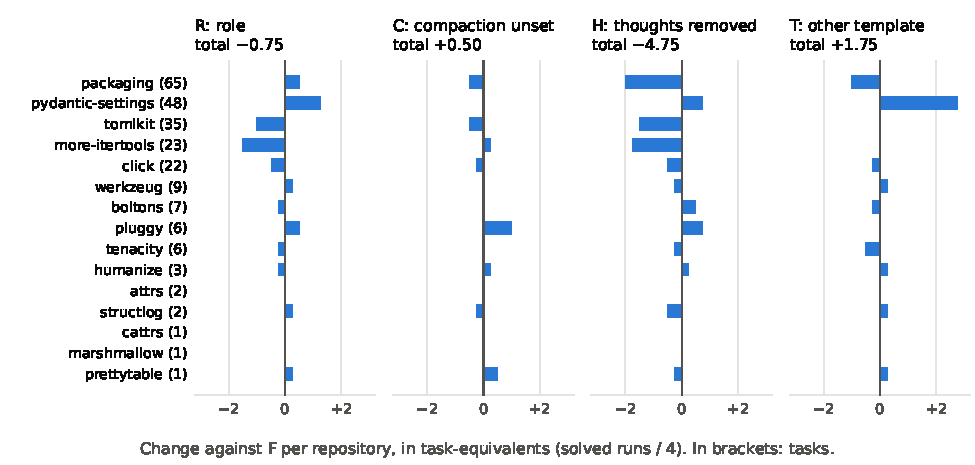
\includegraphics[width=\linewidth]{fig/supp_repos.pdf}
\caption{Change against F in each repository, per arm. Repositories are ordered by their number of tasks.}
\label{fig:s-repos}
\end{figure}

\subsection{Sensitivity analyses}

Three sensitivity analyses were registered with the primary one (Table~\ref{tab:s-sens}). The first treats the runs
that were unsolved at the five-minute limit as missing, in both arms; the estimate of H is then $\SHTimeCapMissing$
points ($p = \SHTimeCapMissingP$) instead of $-\SHd$. The other two score as unsolved every slot whose first job was
interrupted, in the arm or in F. No sensitivity analysis gives a $p$-value below 0.05.

\begin{table}[!htb]
\centering
\caption{Pre-registered sensitivity analyses of the primary estimate (percentage points; exact two-sided sign-flip $p$, unadjusted).}\label{tab:s-sens}
\footnotesize
\begin{tabular}{llrrrr}
\toprule
Arm & Analysis & Tasks & Runs affected & $d$ & Exact $p$ \\
\midrule
R & five-minute-limit runs of both arms treated as missing & 229 & 37 & ${-}0.29$ & 0.8652 \\
 & slots of the arm with an infrastructure row scored unsolved & 231 & 5 & ${-}0.43$ & 0.8011 \\
 & slots of F with an infrastructure row scored unsolved & 231 & 3 & ${-}0.22$ & 0.9321 \\
C & five-minute-limit runs of both arms treated as missing & 229 & 34 & ${+}0.22$ & 0.9253 \\
 & slots of the arm with an infrastructure row scored unsolved & 231 & 5 & ${+}0.11$ & 1.0000 \\
 & slots of F with an infrastructure row scored unsolved & 231 & 3 & ${+}0.32$ & 0.8506 \\
H & five-minute-limit runs of both arms treated as missing & 226 & 123 & ${-}1.25$ & 0.3414 \\
 & slots of the arm with an infrastructure row scored unsolved & 231 & 8 & ${-}2.16$ & 0.0980 \\
 & slots of F with an infrastructure row scored unsolved & 231 & 3 & ${-}1.95$ & 0.1270 \\
T & five-minute-limit runs of both arms treated as missing & 229 & 36 & ${+}0.76$ & 0.5604 \\
 & slots of the arm with an infrastructure row scored unsolved & 231 & 3 & ${+}0.76$ & 0.5604 \\
 & slots of F with an infrastructure row scored unsolved & 231 & 3 & ${+}0.87$ & 0.4947 \\
\bottomrule
\end{tabular}
\end{table}


\subsection{Exposure and the prompt check}

A divergence can only matter in the requests it changes. The frozen checker re-rendered all \SRequests{} returned
requests from the request dumps of the jobs. For each of the \SChecksPassed{} analysed runs it confirmed that the
prompts carry the divergence of the run's arm and no other difference; \SChecksFailed{} runs failed the check. The
divergence changed \SExposureMin{} to \SExposureMax\% of the requests in R, H and T, and \SCChanged\% in C
(Table~\ref{tab:s-exposure}).

\begin{table}[!htb]
\centering
\caption{Exposure: requests re-rendered by the frozen checker, and those whose rendered prompt the arm's divergence changed.}\label{tab:s-exposure}
\footnotesize
\begin{tabular}{lrrrrr}
\toprule
Arm & Runs & Requests checked & Changed by the divergence & Share (\%) & Failed calls recorded \\
\midrule
F & 924 & 15{,}043 & 0 & 0.0 & 17 \\
R & 924 & 15{,}290 & 13{,}616 & 89.1 & 20 \\
C & 924 & 13{,}036 & 2{,}709 & 20.8 & 131 \\
H & 924 & 17{,}450 & 15{,}684 & 89.9 & 112 \\
T & 924 & 14{,}787 & 12{,}629 & 85.4 & 19 \\
\bottomrule
\end{tabular}

\par\smallskip\parbox{0.96\linewidth}{\footnotesize No run has more than one failed call. Of the 299 failed calls, 178 are in runs unsolved at the five-minute limit, 115 in runs that ended on a rejected over-long prompt and 6 in solved runs.}
\end{table}


\subsection{Exploratory run measures}

Table~\ref{tab:s-measures} compares thirteen measures of a run between each arm and F. These comparisons were not
part of the registered tests and are not adjusted for multiplicity. H runs are longer: \SHTimeMean{}~s of agent time
on average against \SFTimeMean{}~s in F (medians \SHTimeMedian{} and \SFTimeMedian{}~s; Figure~\ref{fig:s-time}), with
\SHTokOut{} completion tokens per run against \SFTokOut.

\begin{table}[!htb]
\centering
\caption{Exploratory run measures: mean in arm F, and the paired difference of each arm against F; below it, its 95\% interval (CR1, repository clusters). No multiplicity adjustment.}\label{tab:s-measures}
\footnotesize\setlength{\tabcolsep}{3.5pt}
\begin{tabular}{lrrrrr}
\toprule
Measure & F mean & R $-$ F & C $-$ F & H $-$ F & T $-$ F \\
\midrule
history summaries per run & 0.69 & ${+}0.13$ & ${-}0.69$ & ${-}0.30$ & ${-}0.02$ \\
 &  & {\scriptsize [${+}0.04$, ${+}0.22$]} & {\scriptsize [${-}0.86$, ${-}0.53$]} & {\scriptsize [${-}0.47$, ${-}0.12$]} & {\scriptsize [${-}0.10$, ${+}0.06$]} \\[-2pt]
\addlinespace[2pt]% \\
runs with a summary (share) & 0.482 & ${+}0.038$ & ${-}0.482$ & ${-}0.161$ & ${-}0.014$ \\
 &  & {\scriptsize [${-}0.024$, ${+}0.099$]} & {\scriptsize [${-}0.572$, ${-}0.391$]} & {\scriptsize [${-}0.249$, ${-}0.073$]} & {\scriptsize [${-}0.059$, ${+}0.030$]} \\[-2pt]
\addlinespace[2pt]% \\
largest prompt (tokens) & 12{,}721 & ${+}220$ & ${+}2{,}160$ & ${-}1{,}499$ & ${-}95$ \\
 &  & {\scriptsize [${+}111$, ${+}329$]} & {\scriptsize [${+}1{,}666$, ${+}2{,}655$]} & {\scriptsize [${-}1{,}903$, ${-}1{,}095$]} & {\scriptsize [${-}284$, ${+}95$]} \\[-2pt]
\addlinespace[2pt]% \\
over-long prompt rejected (share) & 0.000 & ${+}0.000$ & ${+}0.123$ & ${+}0.001$ & ${+}0.000$ \\
 &  & {\scriptsize [${+}0.000$, ${+}0.000$]} & {\scriptsize [${+}0.075$, ${+}0.172$]} & {\scriptsize [${-}0.001$, ${+}0.003$]} & {\scriptsize [${+}0.000$, ${+}0.000$]} \\[-2pt]
\addlinespace[2pt]% \\
five-minute limit (share) & 0.018 & ${+}0.003$ & ${+}0.000$ & ${+}0.096$ & ${+}0.002$ \\
 &  & {\scriptsize [${-}0.005$, ${+}0.012$]} & {\scriptsize [${-}0.005$, ${+}0.005$]} & {\scriptsize [${+}0.073$, ${+}0.119$]} & {\scriptsize [${-}0.002$, ${+}0.006$]} \\[-2pt]
\addlinespace[2pt]% \\
tool-call budget reached (share) & 0.006 & ${+}0.003$ & ${-}0.005$ & ${+}0.013$ & ${-}0.002$ \\
 &  & {\scriptsize [${-}0.004$, ${+}0.011$]} & {\scriptsize [${-}0.012$, ${+}0.001$]} & {\scriptsize [${-}0.002$, ${+}0.028$]} & {\scriptsize [${-}0.006$, ${+}0.002$]} \\[-2pt]
\addlinespace[2pt]% \\
no submission (share) & 0.005 & ${-}0.004$ & ${-}0.003$ & ${-}0.004$ & ${+}0.001$ \\
 &  & {\scriptsize [${-}0.015$, ${+}0.006$]} & {\scriptsize [${-}0.013$, ${+}0.007$]} & {\scriptsize [${-}0.015$, ${+}0.006$]} & {\scriptsize [${-}0.010$, ${+}0.012$]} \\[-2pt]
\addlinespace[2pt]% \\
agent time (s) & 77.8 & ${+}3.9$ & ${-}11.2$ & ${+}58.9$ & ${-}1.2$ \\
 &  & {\scriptsize [${-}0.1$, ${+}7.9$]} & {\scriptsize [${-}14.7$, ${-}7.8$]} & {\scriptsize [${+}49.4$, ${+}68.3$]} & {\scriptsize [${-}6.5$, ${+}4.0$]} \\[-2pt]
\addlinespace[2pt]% \\
model calls & 16.28 & ${+}0.27$ & ${-}2.17$ & ${+}2.60$ & ${-}0.28$ \\
 &  & {\scriptsize [${-}0.25$, ${+}0.79$]} & {\scriptsize [${-}2.51$, ${-}1.83$]} & {\scriptsize [${+}1.31$, ${+}3.90$]} & {\scriptsize [${-}1.05$, ${+}0.50$]} \\[-2pt]
\addlinespace[2pt]% \\
failed model calls & 0.018 & ${+}0.003$ & ${+}0.123$ & ${+}0.103$ & ${+}0.002$ \\
 &  & {\scriptsize [${-}0.005$, ${+}0.012$]} & {\scriptsize [${+}0.077$, ${+}0.169$]} & {\scriptsize [${+}0.079$, ${+}0.127$]} & {\scriptsize [${-}0.002$, ${+}0.006$]} \\[-2pt]
\addlinespace[2pt]% \\
tool calls & 12.87 & ${+}0.19$ & ${-}1.23$ & ${+}2.52$ & ${-}0.23$ \\
 &  & {\scriptsize [${-}0.31$, ${+}0.70$]} & {\scriptsize [${-}1.42$, ${-}1.05$]} & {\scriptsize [${+}1.64$, ${+}3.41$]} & {\scriptsize [${-}0.92$, ${+}0.45$]} \\[-2pt]
\addlinespace[2pt]% \\
prompt tokens, summed & 136{,}123 & ${+}3{,}585$ & ${+}9{,}332$ & ${+}12{,}785$ & ${-}3{,}332$ \\
 &  & {\scriptsize [${-}1{,}493$, ${+}8{,}662$]} & {\scriptsize [${+}4{,}824$, ${+}13{,}841$]} & {\scriptsize [${+}443$, ${+}25{,}127$]} & {\scriptsize [${-}11{,}389$, ${+}4{,}725$]} \\[-2pt]
\addlinespace[2pt]% \\
completion tokens & 7{,}690 & ${+}440$ & ${-}1{,}253$ & ${+}6{,}707$ & ${-}245$ \\
 &  & {\scriptsize [${-}18$, ${+}899$]} & {\scriptsize [${-}1{,}635$, ${-}871$]} & {\scriptsize [${+}5{,}645$, ${+}7{,}768$]} & {\scriptsize [${-}796$, ${+}305$]} \\
\bottomrule
\end{tabular}
\end{table}


\begin{figure}[!htb]
\centering
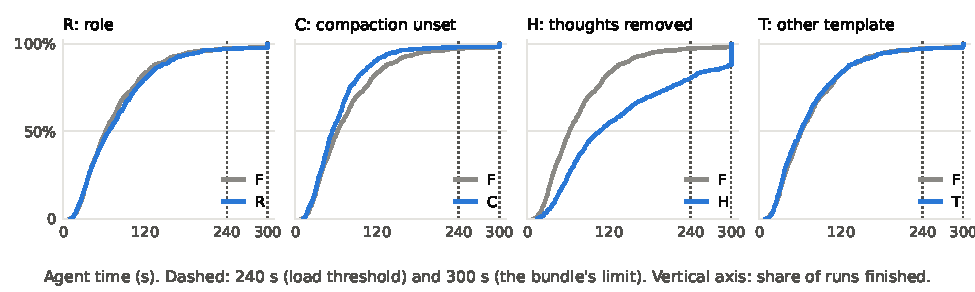
\includegraphics[width=\linewidth]{fig/supp_time.pdf}
\caption{Agent time per run: each arm (blue) against F (grey).}
\label{fig:s-time}
\end{figure}


\subsection{What the case study does and does not show}

The four divergences are not small edits. Three of them change between 85\% and 90\% of all requests of a run, and
one removes the model's earlier reasoning from every request. Yet the simultaneous intervals exclude a loss of more
than \SHSimLo{} points and a gain of more than \STSimHi{} points for any of them. For E4B on these tasks, the
solved share is insensitive to prompt details that we had expected to matter, and that public discussion treats as
traps.

Three limits apply. First, the result holds for this model, this agent bundle and these 15 repositories; we did not
run the experiment with the 31B model. Second, the arm without history thoughts shows the largest estimate, takes
almost twice as long per run and ends at the time limit more often. Its estimate therefore depends on the time
limit: with the time-limit rows treated as missing it is $-1.3$ instead of $-2.1$ points. Third, an insensitive solved
share does not make conformance checks useless. A check is cheap, and it removes a question that otherwise needs
4,620 jobs to answer.

The case study also calibrates the rest of this paper. Its reference arm solved 23.8\% of its runs, and with 924 runs per arm the 95\% interval of each difference
reaches 2.2 to 2.5 points to either side of the estimate. A difference between two E4B arms that
is to be seen needs this order of size, and \cref{sec:programmes} shows what happens with fewer runs.
